\newpage
\section{GD CAD}
The GD-CAD project is a CAD drawing tool.It is working tool. It is working natively using Qt.

\subsection{GUI in GDCAD}
Implementation of the coding interface of the GDCAD in which user can draw the codes using 
command line. The interface is Dokable, can be movable ,minimized. It is able to perform all 
the basic operation of load ,Save , SaveAs.\\
\begin{figure}[!htb]
\centering
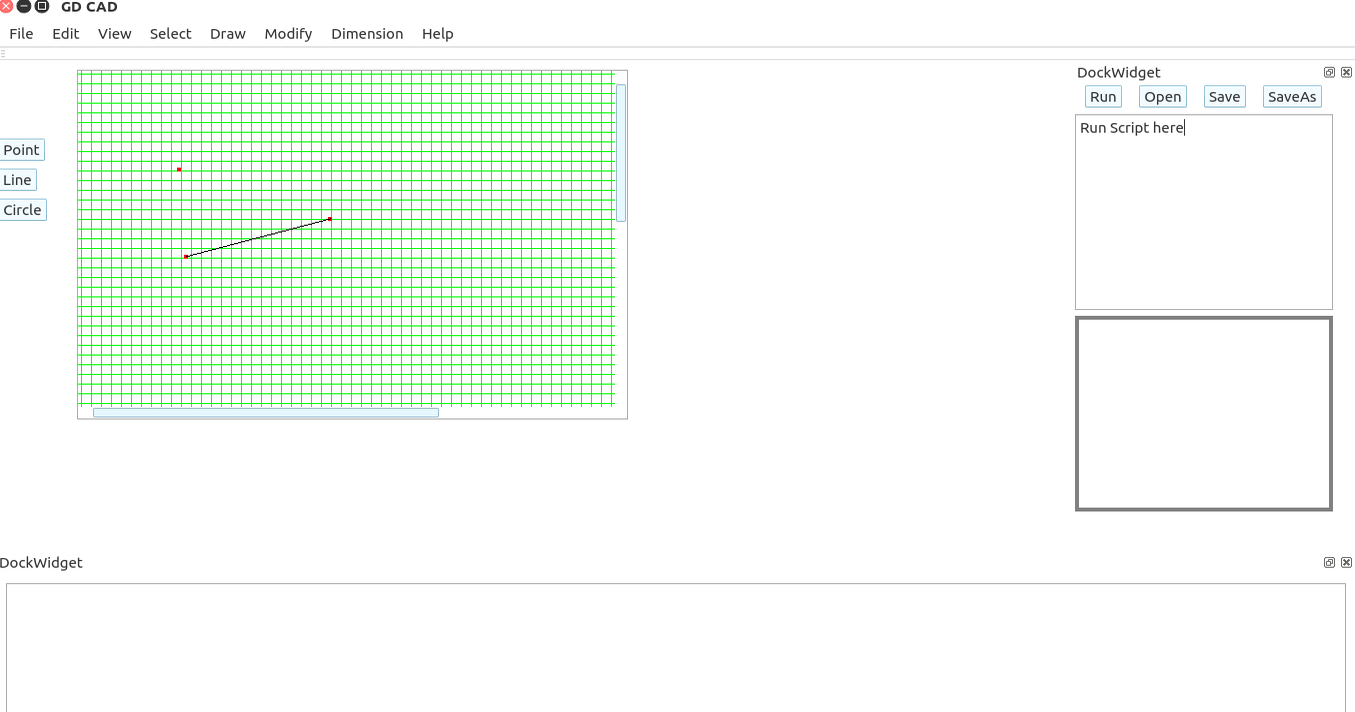
\includegraphics[scale=0.3]{images/dp/gdc.png}                   
\vspace{-1em}
\caption{GD CAD GUI (Graphic User Interface)}
\hspace{-1.5em}
\end{figure}
